\documentclass[10pt,letterpaper]{article}

\usepackage{cogsci}
\usepackage{pslatex}
\usepackage[nodoi]{apacite}
\usepackage{graphicx}
%\graphicspath{plots/}
%\usepackage{float}
\usepackage[font=small]{caption}
\usepackage{subcaption}
\usepackage{lipsum}
\usepackage[section]{placeins}


\title{Developmental Change in the Relationship Between Lexical and Grammatical Acquisition}
 
\author{{\large \bf Mika Braginsky} \\
  \texttt{mikabr@stanford.edu} \\
  Department of Psychology \\
  Stanford University
  \And {\large \bf Daniel Yurovsky} \\
  \texttt{yurovsky@stanford.edu} \\
  Department of Psychology \\
  Stanford Uiversity
    \And {\large \bf Virginia Marchman} \\
    \texttt{marchman@stanford.edu} \\
  Department of Psychology \\
  Stanford Uiversity
    \And {\large \bf Michael C. Frank}\\
    \texttt{mcfrank@stanford.edu} \\
  Department of Psychology \\
  Stanford Uiversity}


\begin{document}

\maketitle

\begin{abstract}
\lipsum[1]

\textbf{Keywords:} 
foo; bar; baz
\end{abstract}

\section{Introduction}

[Intro material written by Mike:]
Does abstract structure in language emerge from the interaction of individual words, or are syntactic structures represented separately? On lexicalist theories of grammatical development, syntactic structure emerges from graded generalizations on the basis of lexical items and there may be little or no representation of syntactic rules or regularities per se, at least early in development \cite{tomasello2001,tomasello2003}. Even if syntactic structures are eventually represented, these representations should be directly related to their support in more concrete lexical structure \cite{bannard2009,bod2010}. In contrast, on theories like principles and parameters, grammar is predicted to emerge independently from lexical knowledge and on its own (largely maturational) timetable. On these theories, older children should have more syntactic competence, largely independent from the amount of language input they receive and hence from the size of their vocabulary.

Developmental data can help resolve this conflict by providing estimates of the relationship between grammar, lexicon, and age. Indeed, in a now-classic set of analyses, \cite{bates1994} showed a systematic relationship between ...

[Intro material written by Mika:]
[Sentence about how all grammar generalizations must involve both input and internal stuff]. However, theories of grammatical development differ in the role that they assign to experience and internal processes and the emphasis that they place on one or the other. One one hand, in the more nativist and domain-specific tradition [stuff about generative grammar and Principles and Parameters (cite Atoms of Language and Chomsky); basically everything is maturation]. On the other hand, [stuff about emergentism and lexicalist grammar \cite{bates1999} and maybe some Tomasello)].

[Stuff about how those theories make different predictions and how those predictions can be explored in empirical studies of lexicon-grammar relationship. If there's age-related change, functions should be different at different age points. If there's no age-related change, functions should be the same.]

[What functions? How two relate lexicon to grammatical development? Two different metrics: 1) usage of grammatical forms and constructions; 2) composition of lexicon by grammatical function.]

[How to measure any of these things? CDI of course! Justification for CDI \cite{fenson1994}, justification for complexity section \cite{dale1991,dale1989} and word form section (???).]

[Previous work on lexicon-grammar: well-established tight connection between lexicon and grammar, same non-linear function everywhere]. [Bates and Goodman (1999) conclude that grammar is entirely predictable from lexicon. But we find additional effect of age, suggesting there's a tight link but there's also something developmental going on.]

[Previous work on lexical composition: English \cite{bates1994}, other languages (???).]

\clearpage

\section{General Methods}

TODO: some text here

\subsection{CDI Form Database}

We implemented Wordbank (\texttt{wordbank.stanford.edu}), a structured database of CDI data, to aggregate and archive CDI data across languages and labs. By collecting language development data at an unprecedented scale, Wordbank enables the exploration of novel hypotheses about the course of lexical and grammatical development. [TODO: more about wordbank? what's useful?]

Wordbank now includes data in four languages: English, Spanish, Norwegian \cite{kristoffersen2013,simonsen2014}, and Danish \cite{andersen2006}, including both cross-sectional and longitudinal data.
%Table \ref{table:num} breaks down our data by language in terms of the total number of administrations of the CDI and the number of administrations that include grammar (word form and complexity) data.
[TODO: more about how/where data came from?]

%\begin{table}
%\begin{center}
%\begin{tabular}{| l | r | r |}
%\hline
%& Administrations & with Grammar\\ \hline
%English & 5595 & 4137\\ \hline
%Spanish & 1094 & 1094\\ \hline
%Norwegian & 10095 & 8505\\ \hline
%Danish & 3038 & 2074\\ \hline
%\end{tabular}
%\caption{TODO}
%\label{table:num}
%\end{center}
%\end{table}

\subsection{CDI Measures}

In general, CDI forms contain both vocabulary checklists and other questions relevant to the child's linguistic development. All of the data used here is from the Words and Sentences (Toddler) CDI instruments of each language. Each of these instruments includes a vocabulary section, which asks whether the child produces each of around 700 words form a variety of semantic and syntactic categories; a word form section, which asks whether the child produces each of around 30 morphologically inflected forms of nouns and verbs; and a complexity section, which asks whether the child's speech is most similar to the syntactically simpler or more complex versions of around 40 sentences. Each language's instrument is not merely a translation of the English words and sentences, but rather constructed and normed specifically to reflect the lexicon and grammar of that language. Table \ref{table:measures} shows, for each language, the number of items in each of these categories [TODO: also include examples of each?].

\begin{table}[b]
\begin{center}
\begin{tabular}{| l | r | r | r |}
\hline
& Vocabulary & Word Form & Complexity\\ \hline
English & 680 & 25 & 37\\ \hline
Spanish & 680 & 24 & 37\\ \hline
Norwegian & 731 & 33 & 42\\ \hline
Danish & 725 & 29 & 33\\ \hline
\end{tabular}
\caption{\label{table:measures} Overview of instruments in each language: number of items in each relevant section.}
\end{center}
\end{table}

To analyze lexical and grammatical development, we derive several quantities based on these measures. Each child's vocabulary size is the proportion of the words on the corresponding CDI form that the child is reported to produce. Similarly, each child's word form score is the proportion of word forms they are reported to produce, and their complexity score the proportion of complexity items for which they are reported to use the more complex form. We compute all of these quantities as proportions rather than numbers of items to make the scales comparable across languages.

\section{Syntax and Morphology}

By the age of two years, most children have a sizable working vocabulary, including verbs, prepositions and closed class forms that perform grammatical work functions  They are also beginning to use two- or three-word combinations (e.g., ``mommy sock'') and may demonstrate productive use of inflectional morphemes (e.g., past tense ``-ed''). As with vocabulary, there is sizable variation in when and how children move into grammar, and children who are more advanced in early vocabulary are more advanced in grammatical development as well \cite{bates1999}. This suggests that the mechanisms guiding vocabulary and grammar learning are highly interdependent \cite{tomasello2003,bresnan2001}, a view at odds with the nativist assumption that grammar emerges independent of the lexicon \cite{chomsky1981}.

Previous studies have found a strong connection between the size of the lexicon and grammatical development as measured by the complexity section of the CDI. A consistent non-linear relationship appears across a variety of languages, including English \cite{bates1994,fenson1994}, Italian \cite{caselli1999}, Hebrew \cite{maital2000}, and Spanish \cite{jackson-maldonado2003}. However, no studies have had the power and cross-linguistic representation to go beyond this initial finding. We extend it by examining grammatical development using two different measures: word form as a window into morphology and complexity as a window into syntax. For each measure, we investigate the interaction of vocabulary size and age in a variety of languages.

\subsection{Analysis}

\begin{figure*}[tb]
\begin{center}
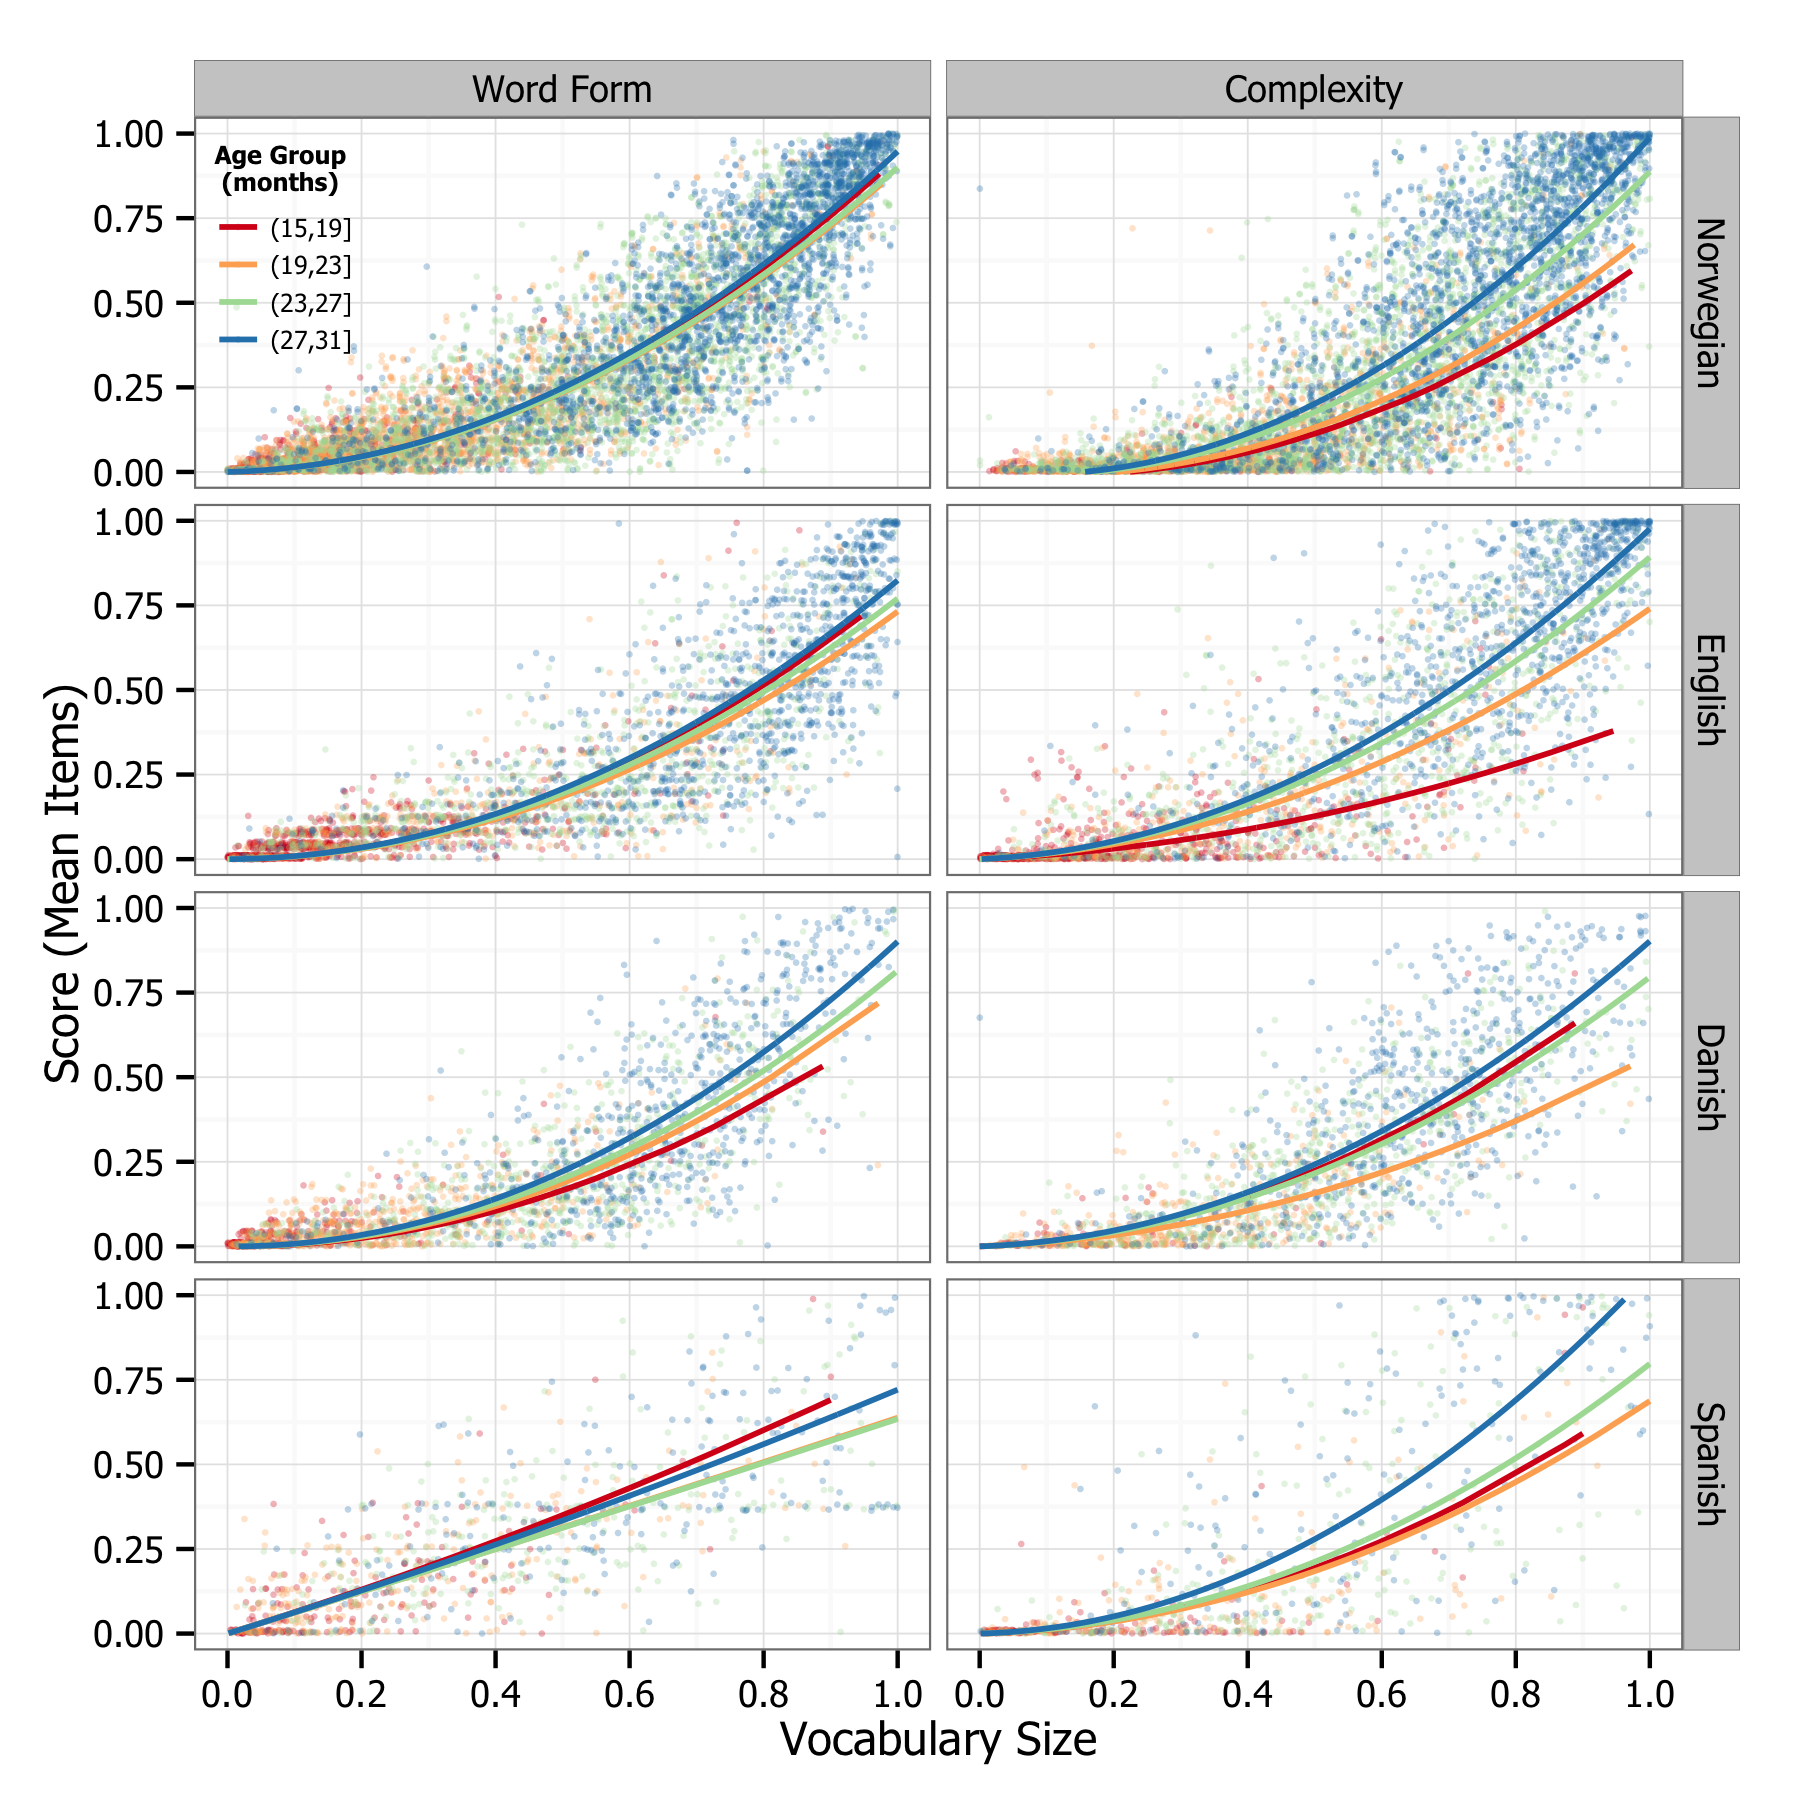
\includegraphics[width=.9\textwidth]{plots/grammar.png}
\end{center}
\caption{\label{fig:grammar} Each point shows an individual child, indicating their total vocabulary size and word form score or complexity score, with color showing their age bin (English $n=4137$; Spanish $n=1094$; Norwegian $n=8505$; Danish $n=2074$). Panels show different languages, and curves are regression models fit separately for each language and measure. The models were specified as \small{\tt{score $\sim$ vocab$^{2}$ * age}}.} 
\end{figure*}

For each language in our sample, we wanted to estimate how much of a child's syntactic and morphological development was left to predicted after knowing that child's vocabulary size. Specifically, we asked whether knowing a child's age provided additional predictive power over and above vocabulary size. To estimate this predictive power of age, we fit regression models to each child's word-form and complexity scores. We modeled each child's score as a quadratic function of vocabulary size and interaction with the child's age in months. Figure~\ref{fig:grammar} shows a scatter plot of these data and models. Each dot represents an individual child's score on each measure, while curves show the relationship between that measure and vocabulary size. As seen most clearly for English and Norwegian, the curves for complexity show a characteristic fan, while the curves for word form do not, suggesting that the relationship between vocabulary size and complexity score is modulated by age, while the relationship between vocabulary size and word form score is not (or is to a lesser extent). The Spanish and Danish data show less of a clear complexity curve fan, possibly because of the relatively small number of data points in the youngest age bin.

Because of the size of our samples, all main effects and interactions were highly significant in each language. To test our prediction---that vocabulary development predicts more of the variability in children's morphological than syntactic development---we compared the coefficients in our models across languages and measures. Figure~\ref{fig:coefs_grammar} shows the interaction between age and vocabulary size for each of these models across languages. In each model, the age-related interaction coefficient is substantially larger for complexity than for word form, indicating that for complexity more than word form.

\begin{figure}[tb]
\begin{center}
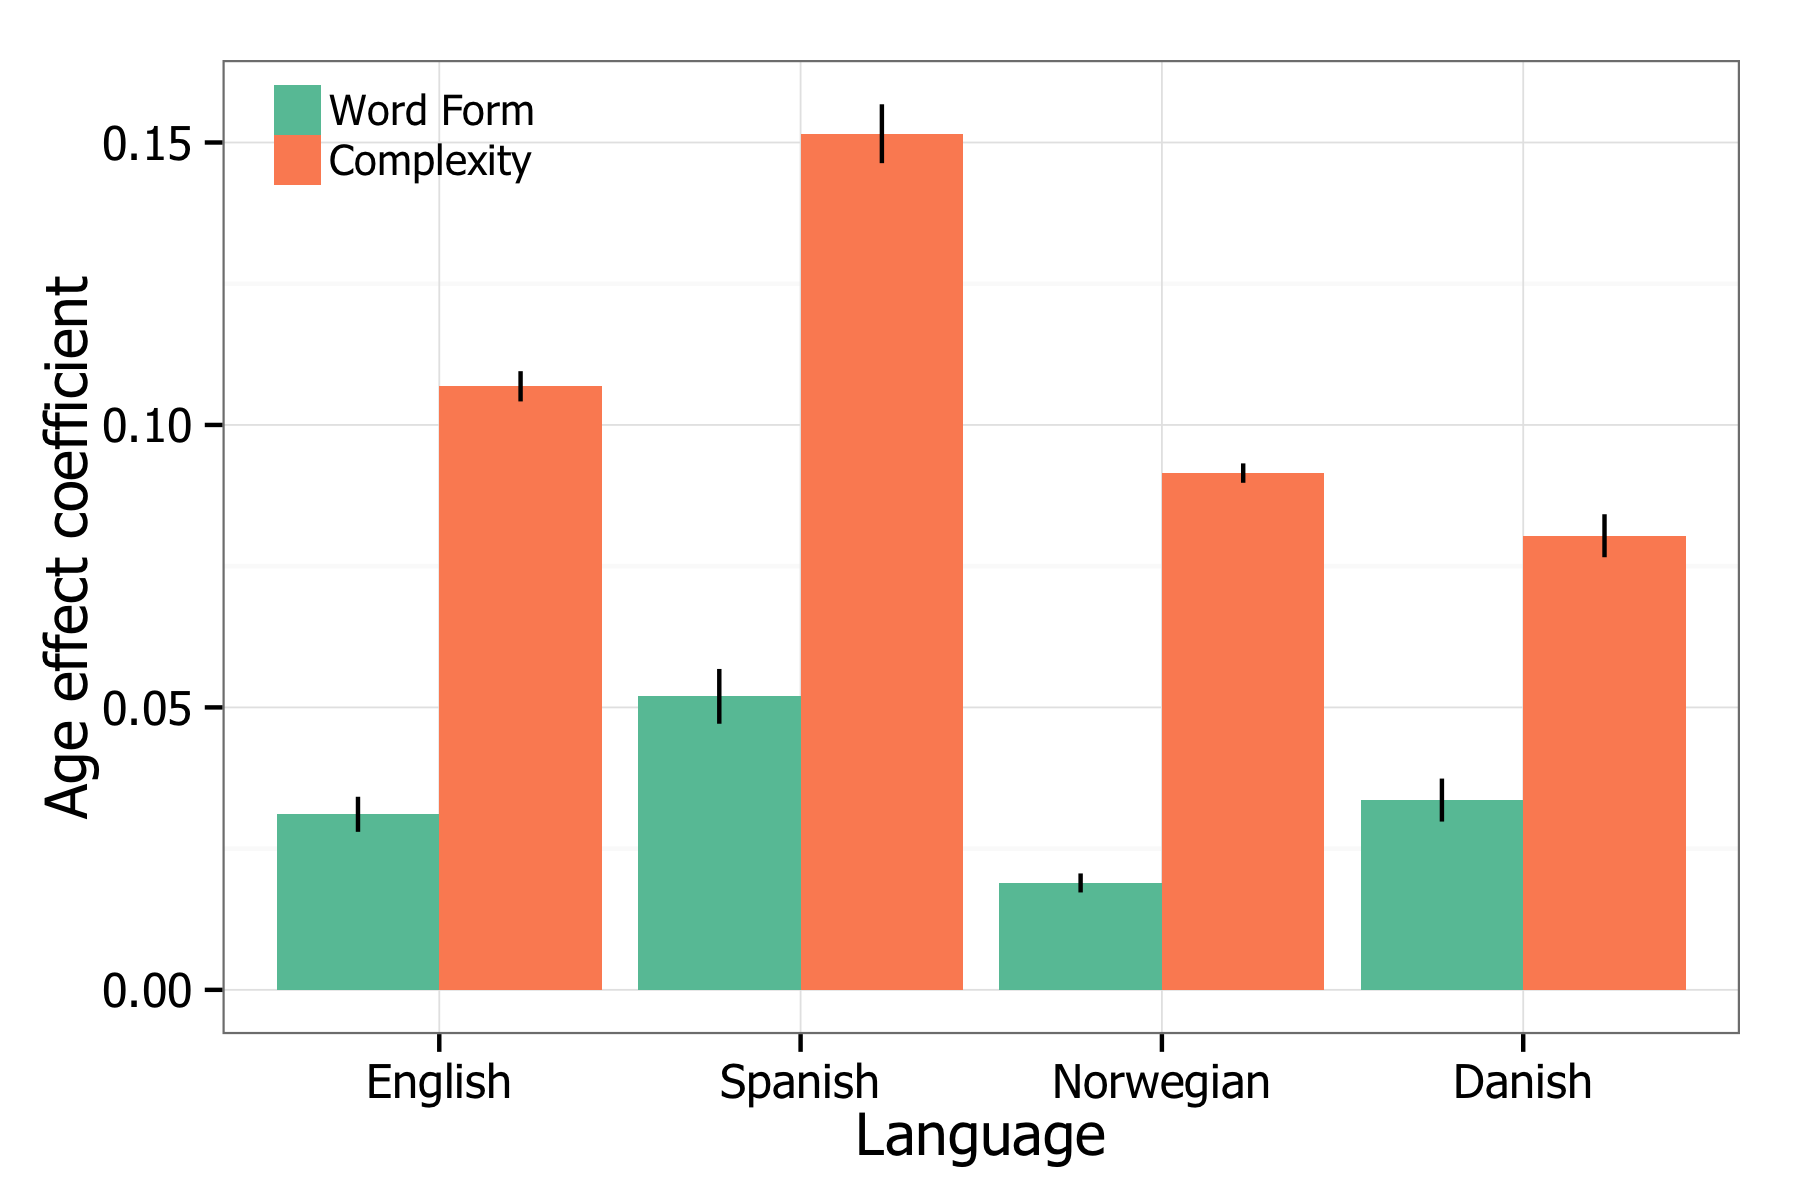
\includegraphics[width=\linewidth]{plots/coefs_wordform_complexity.png}
\end{center}
\caption{\label{fig:coefs_grammar}  For each language and measure (word form and complexity), the coefficient of the interaction between vocabulary size and age. Error bars indicate the $\pm$1SE. Across languages, complexity has a substantially larger interaction with age effect than word form, suggesting that less of children's syntactic development is predicted by their vocabulary growth.} 
\end{figure}

Given the heterogenous nature of the CDI instruments, particularly of the complexity sections, we further break down the items of the complexity sections by classifying them as capturing more morphological or more syntactic phenomena. [TODO: stuff about our coding methods here]. We then fit predictive models as above, but separately for each word form and complexity item. Figure \ref{fig:interactions} shows the z-score ([TODO: why coefficients some places and z-scores other places?]) of the age-interaction terms of the models for each item. [TODO: analyze these results post-coding].

\begin{figure*}[tb]
\centering

\begin{subfigure}[b]{0.45\textwidth}
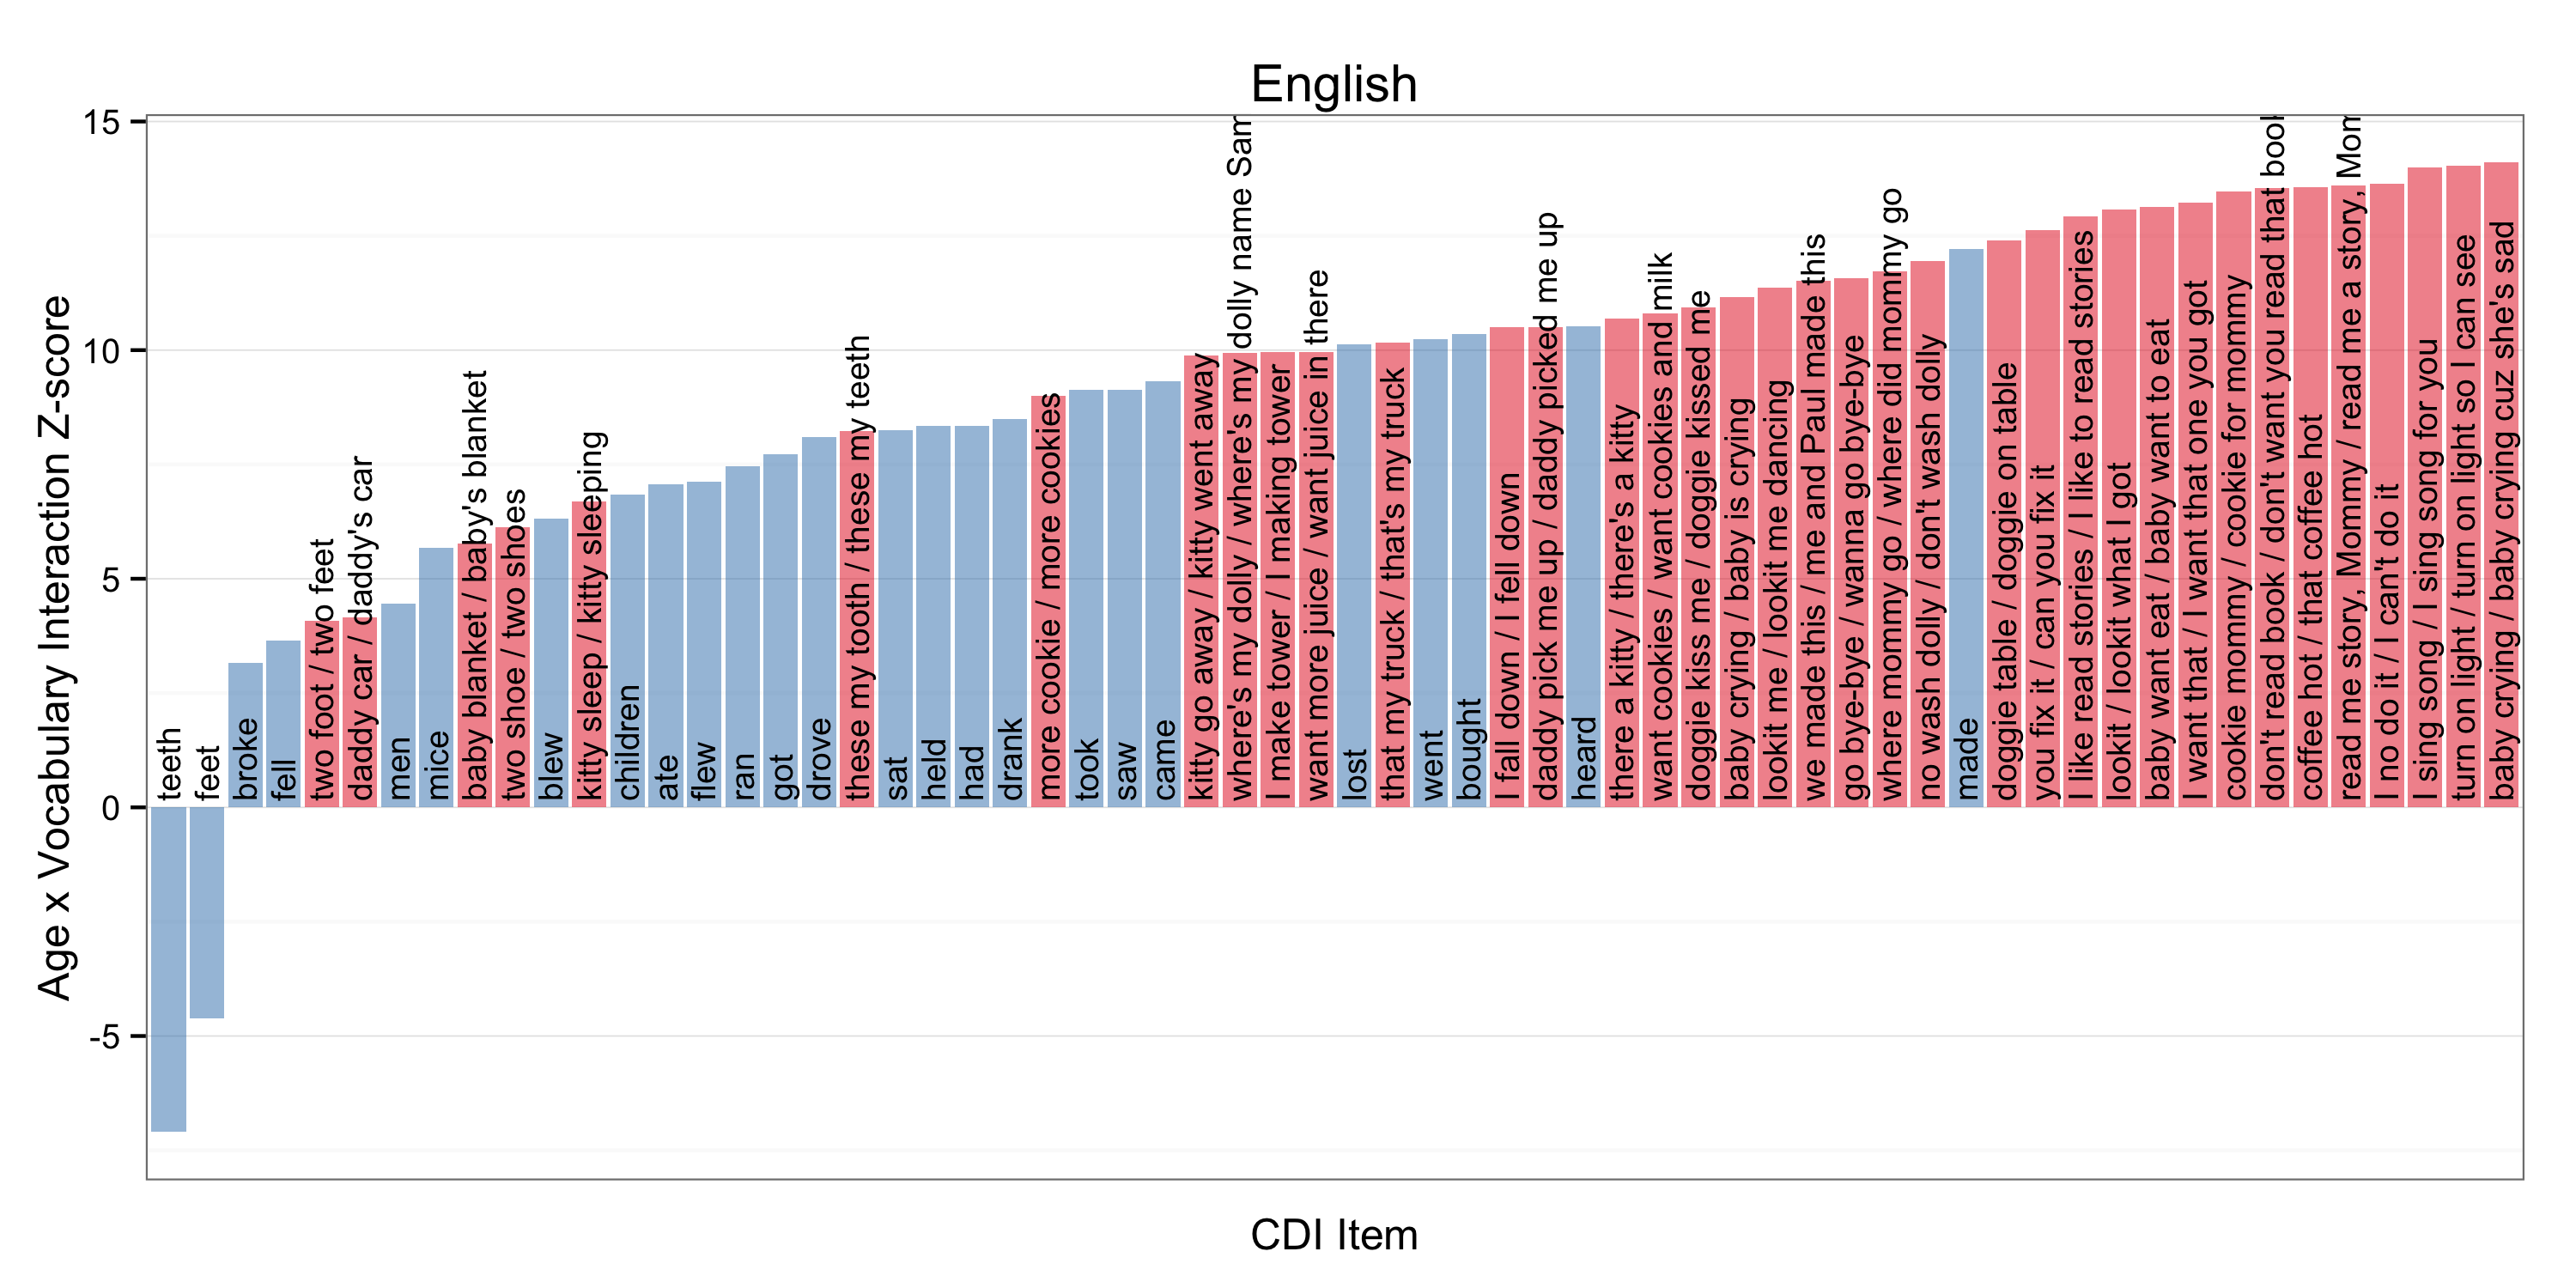
\includegraphics[width=\textwidth]{plots/english_interactions}
\end{subfigure}
\begin{subfigure}[b]{0.45\textwidth}
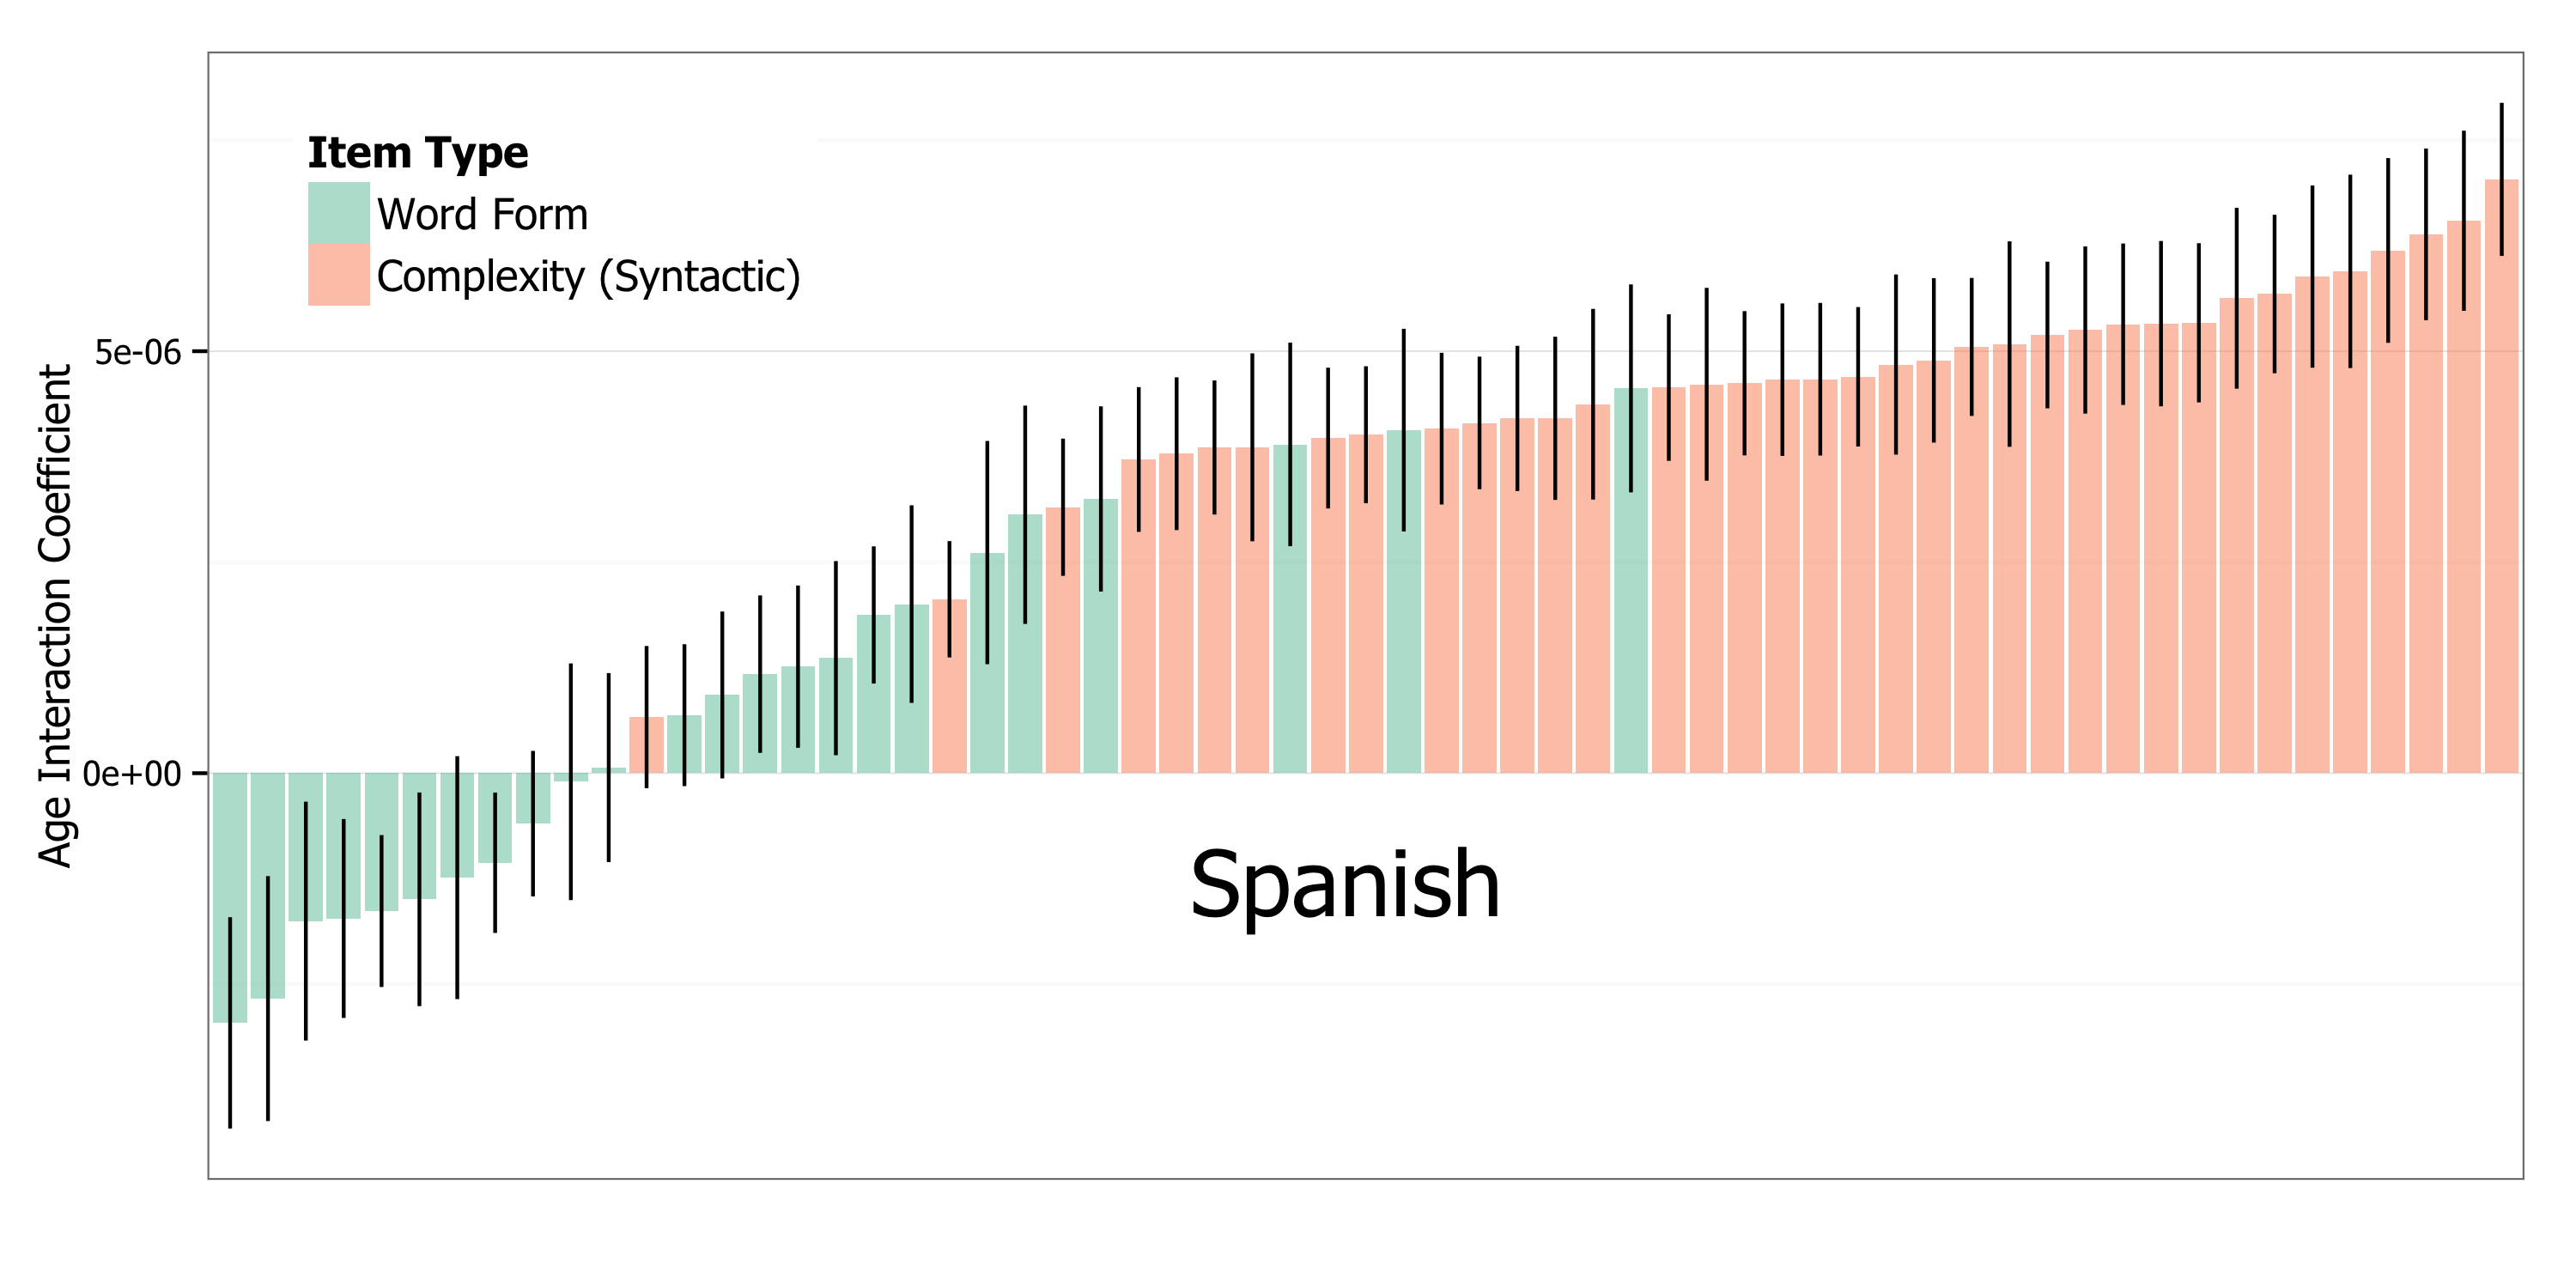
\includegraphics[width=\textwidth]{plots/spanish_interactions}
\end{subfigure}

\begin{subfigure}[b]{0.45\textwidth}
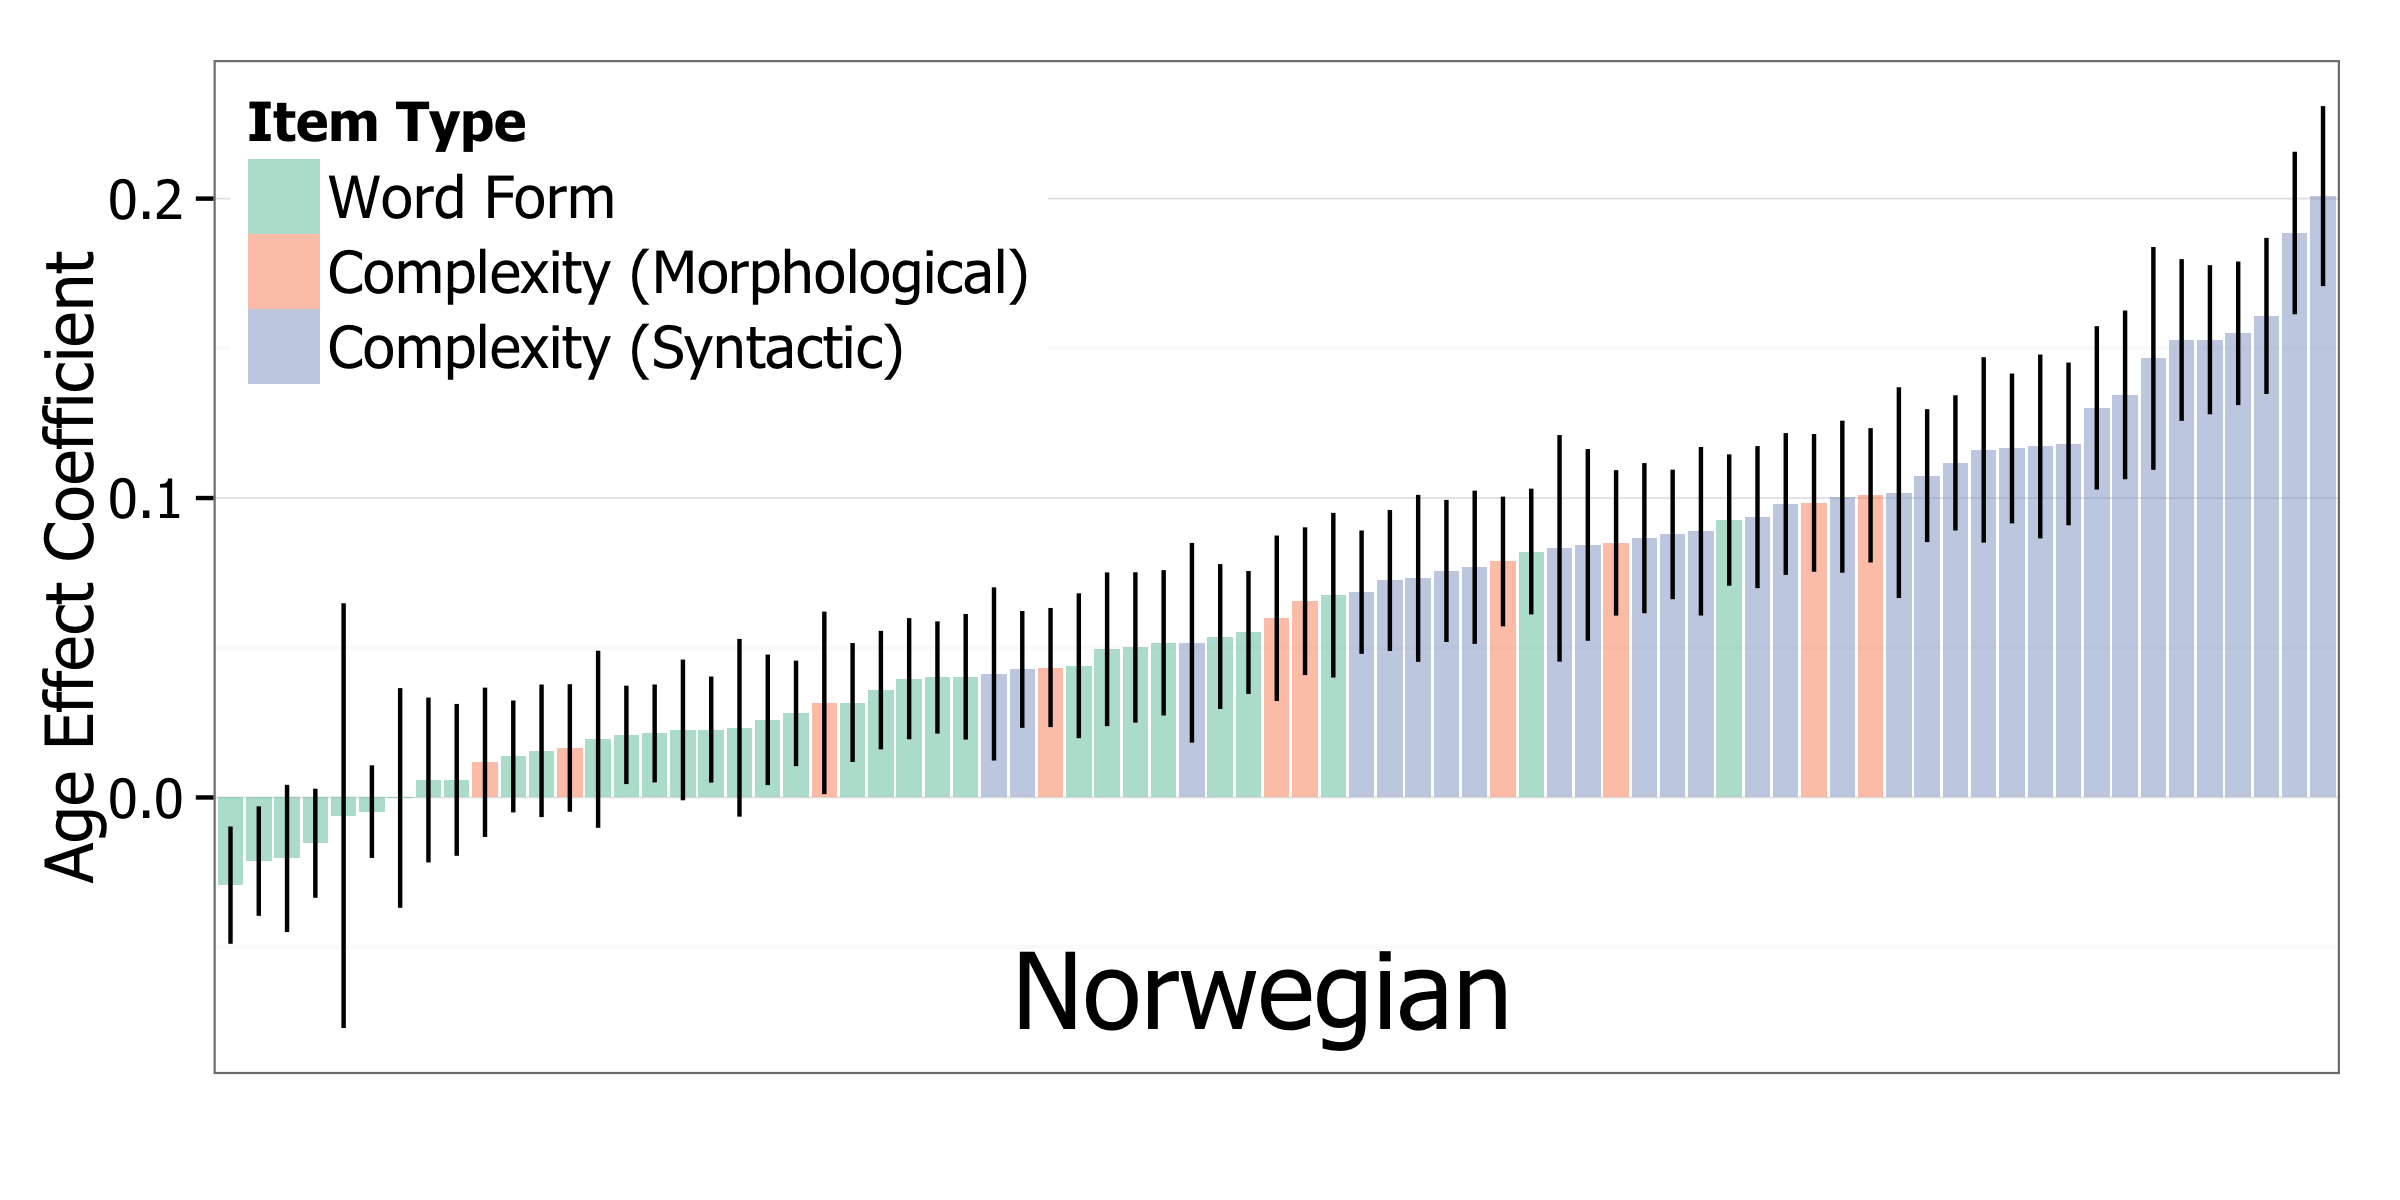
\includegraphics[width=\textwidth]{plots/norwegian_interactions}
\end{subfigure}
\begin{subfigure}[b]{0.45\textwidth}
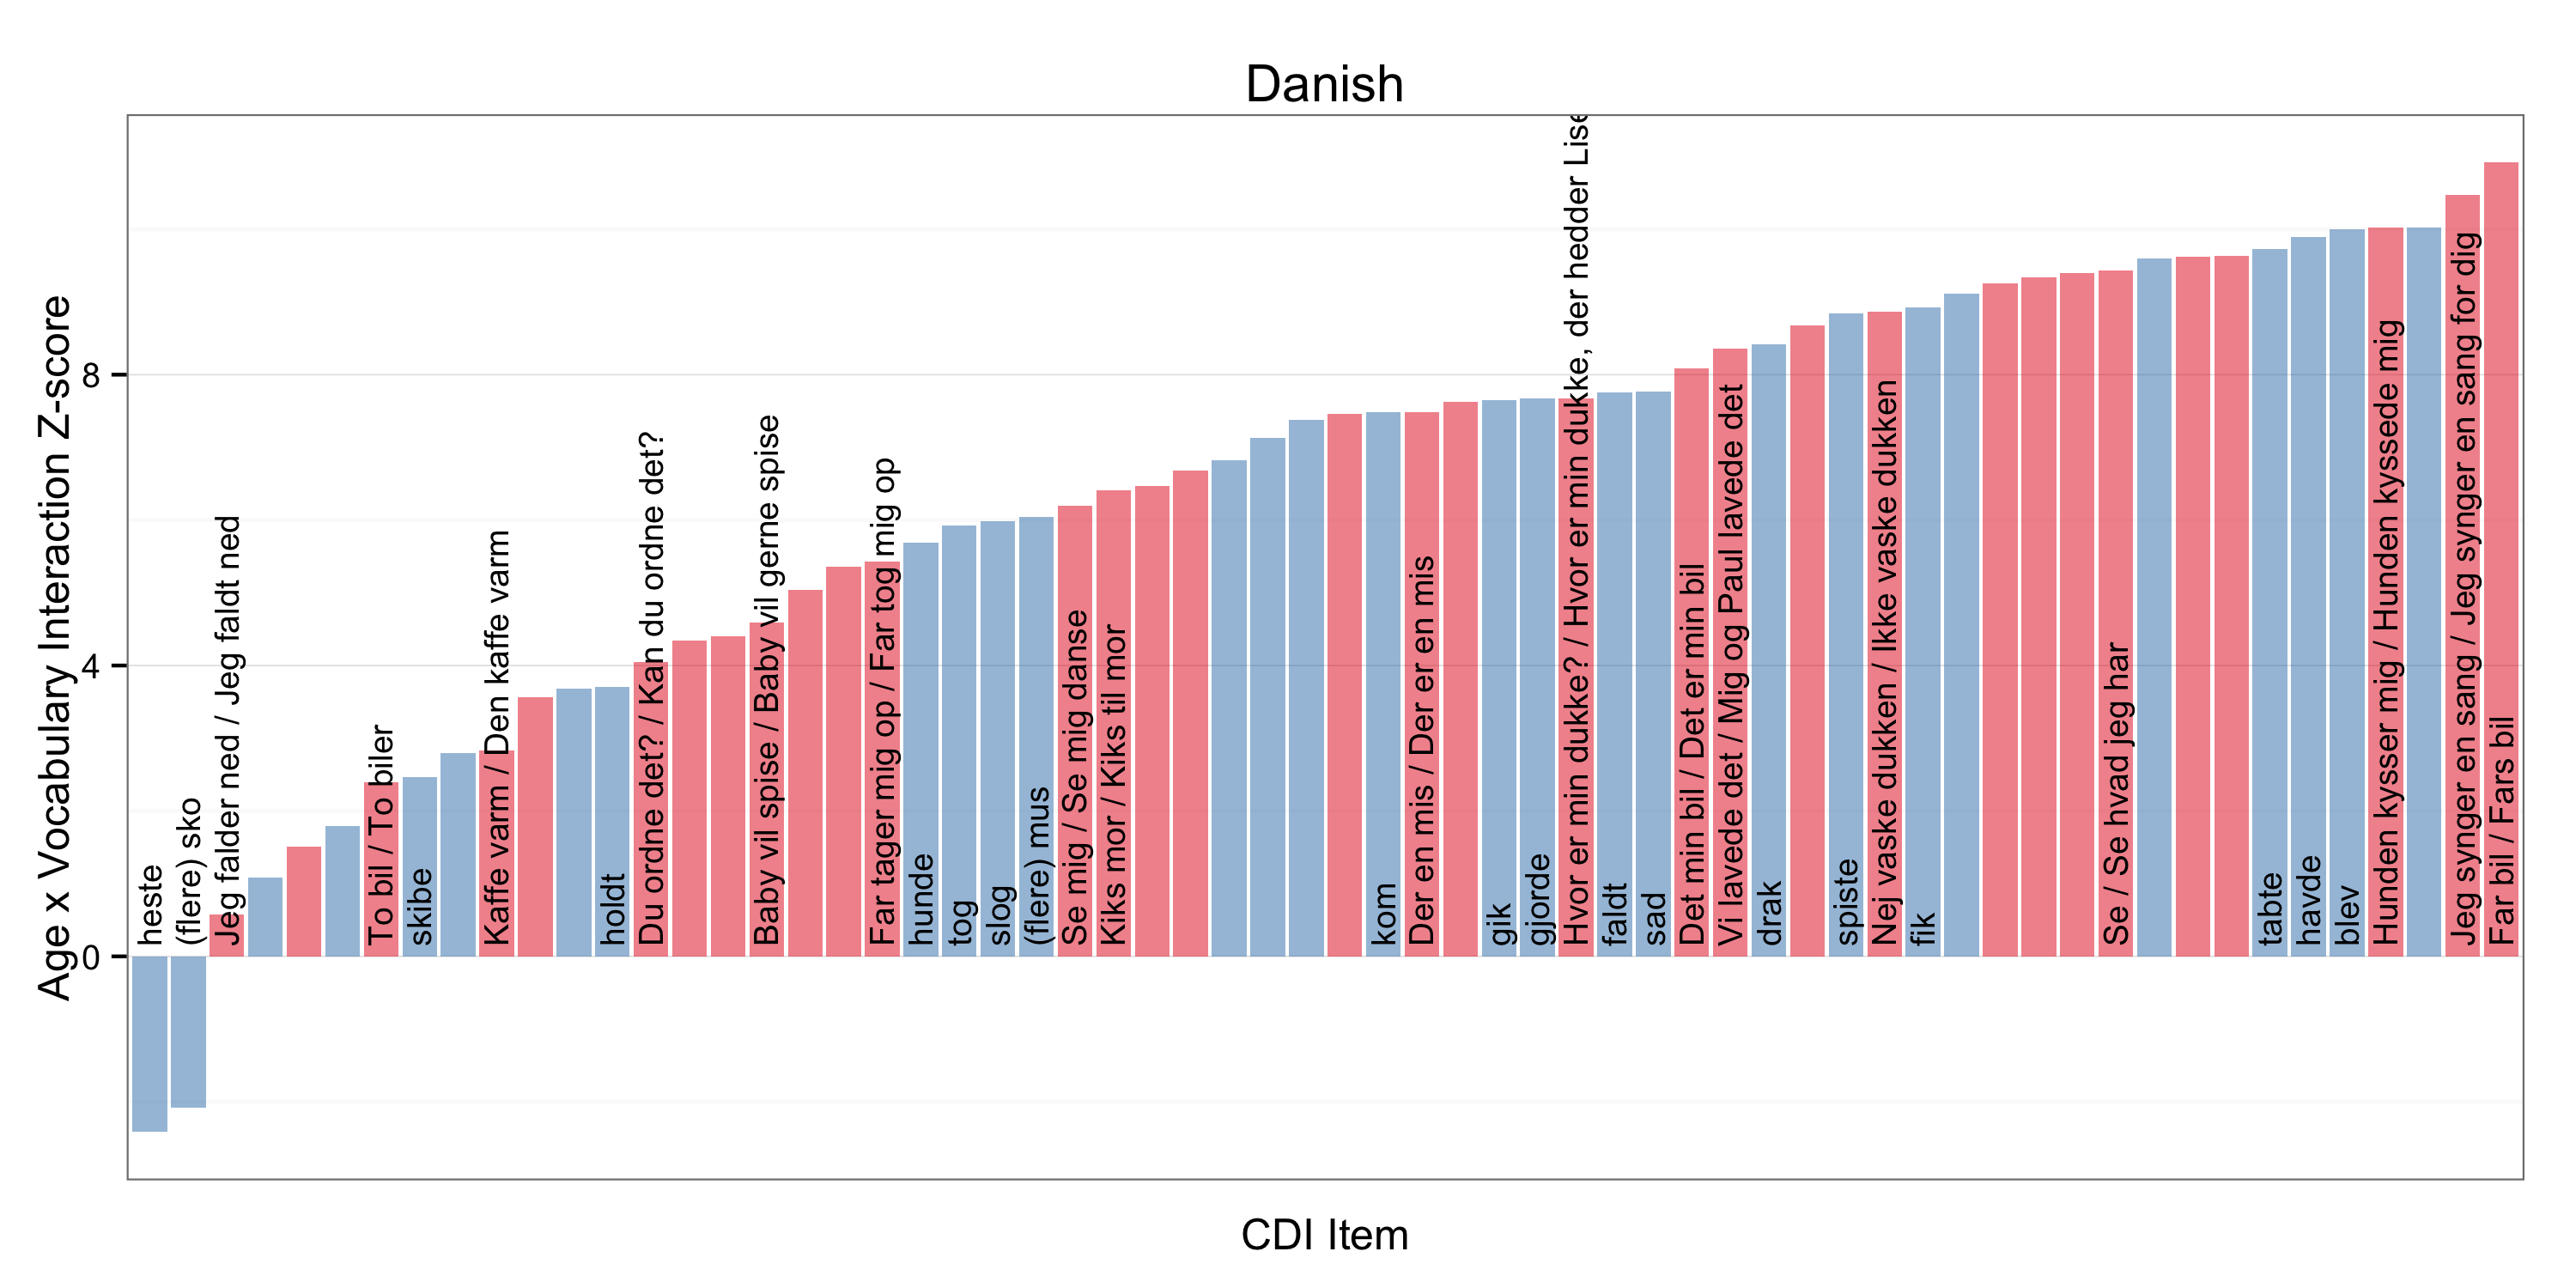
\includegraphics[width=\textwidth]{plots/danish_interactions}
\end{subfigure}

\caption{\label{fig:interactions} For each language and item, the z-score of the model's age and vocabulary size interaction term. Across languages, complexity items tend to have a substantially larger age effect than word form items.}

\end{figure*}

\subsection{Discussion}

We build on previous analyses that showed a strong relationship between lexical and grammatical development, by factoring in the interplay of age with this relationship. We further distinguished in this analyses between measures more reflective of morphology and measures more reflective of syntax, and found that syntactic development broadly shows greater age modulation than morphological development. Thus, this analysis provides circumstantial evidence for the relationship between syntactic development and age, independent of the growth of the lexicon. 

\section{Vocabulary Composition}

Early vocabulary development is typically characterized by learning of names for caregivers and common objects, while later in development, children tend to increase their vocabulary by increasing the proportion of predicates (verbs and adjectives). This over-representation of nouns has been found across a number of analyses and in a variety of languages, though not all \cite{caselli1995}.\footnote{Differences in early vocabulary composition have been argued to emerge from typological differences (e.g., word order, subject drop), and from cultural practices (e.g., focus on picture book reading) \cite{tardif1999, gopnik1996, choi1995}---we are agnostic as to the source of this variability.} For our purposes we are interested in using these analyses of vocabulary composition to test for the same kind of age-related differences that we found in the complexity and word-form analyses reported above. 

We predict that the proportion of verbs in children's vocabulary should be relatively more affected by age than nouns. Concrete nouns are hypothesized to be learned initially from both co-occurrences between words \cite{yu2007b} and by social cues to reference to particular objects \cite{bloom2002}. On neither of these accounts should syntactic information be a primary information source (though of course syntax might be more informative for abstract nouns). In contrast, for verbs, syntax has been argued to be primary in meaningl learning. On the syntactic bootstrapping hypothesis \cite{gleitman1990,fisher1991}, verbs are learned by  mapping the syntactic structure of utterances to the thematic structure of observed events, for example by noticing that the subject of a sentence matches the agent in one particular ongoing event but not another (``the cat is fleeing the dog'' matches  {\sc flees(cat, dog)} but not {\sc chases(dog,cat)}). Thus, if syntactic development is related in some way to age, we should see larger age effects on verb representation than noun representation. 

\subsection{Analysis}

\begin{figure*}[tb]
\begin{center}
\includegraphics[width=\textwidth]{plots/composition.png}
\end{center}
\caption{\label{fig:vocab_comp} Proportion of a particular CDI category, plotted by total vocabulary size. Each point shows an individual child, with color showing their noun, predicate, and function word vocabulary. Panels show different languages, and curves are smoothing functions using loess. (English $n=5595$; Spanish $n=1094$; Norwegian $n=10095$; Danish $n=3038$)} 
\end{figure*}

Each CDI form contains a mixture of words in different classes. We adopt the categorization of \citeA{bates1994}, who split words in nouns, predicates (adjectives, adverbs, and verbs), function words, and other words. Then for each child's vocabulary, we compute the proportion of the total words in each of these categories that they are reported to produce. This yields a set of proportions for each child.

Again following \citeA{bates1994}, for each of the four languages in our sample, we plot these proportions against total vocabulary. These functions are shown in Figure \ref{fig:vocab_comp}: each dot represents an individual child's knowledge of a particular class, while curves show the relationship between that class and the entirety of the vocabulary. If categories grow independently of one another, these curves should approximate the diagonal. This pattern is not what either we or \citeauthor{bates1994} observe however: Across the languages in our sample, nouns are systematically over-represented in smaller vocabularies (shown by a curve that is above the diagonal), while function words---and to some extent, predicates---are under-represented. 

Next, we measure the contribution of age to vocabulary composition. We fit a linear model to all children's data for each word class, predicting word-class proportion as a linear and quadratic (FIXME) function of total vocabulary. We then investigated the interaction between total vocabulary and age. Because of our theoretical interest in the relationship between age and syntactic development, we focus here specifically on nouns and verbs. Figure \ref{fig:coefs_noun_verb} shows coefficients for each of these models across languages. In each model, the age-related interaction coefficient is substantially larger for verbs than for nouns. This asymmetry can be interpreted as evidence that for two vocabulary-matched children, the older would tend to have relatively more verbs than the younger, and this effect was larger for children with overall larger vocabularies.

\begin{figure}[tb]
\begin{center}
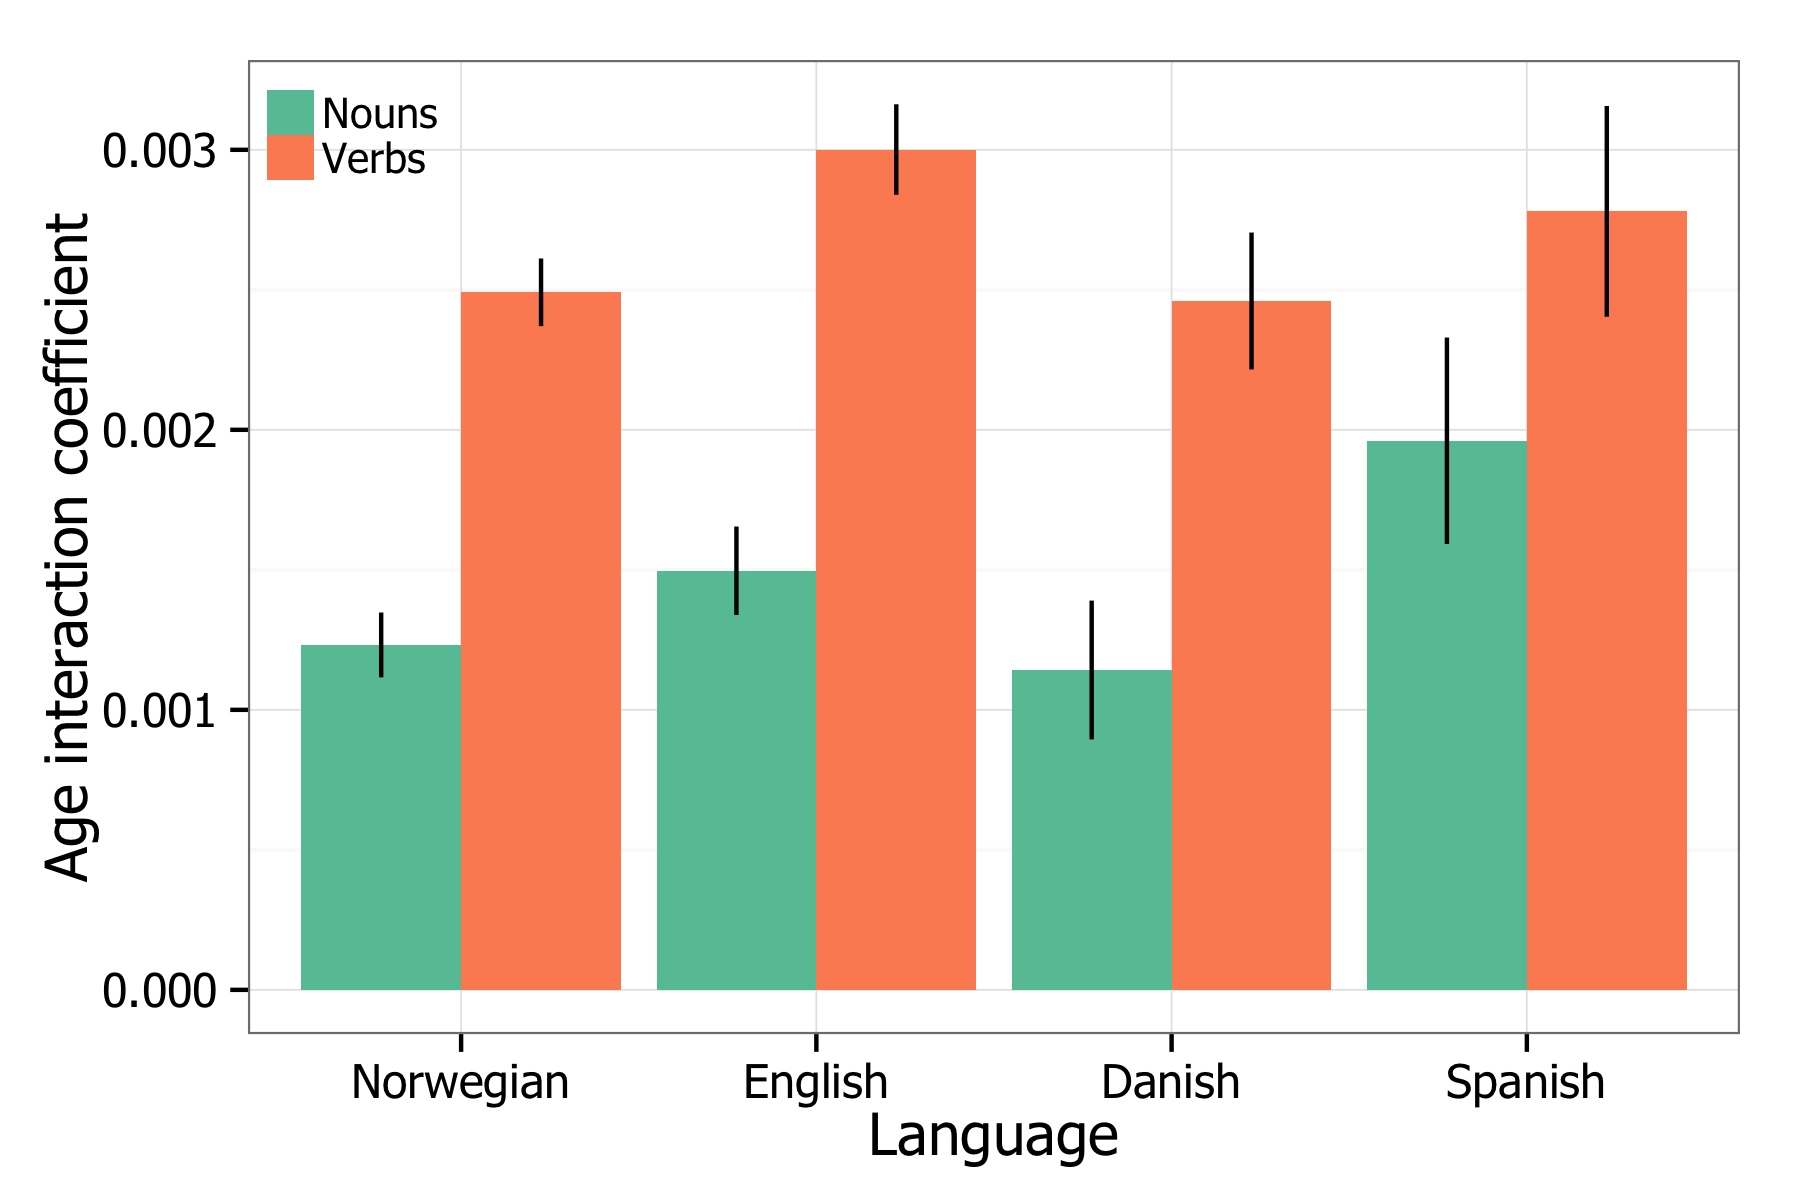
\includegraphics[width=\linewidth]{plots/coefs_noun_verb.png}
\end{center}
\caption{\label{fig:coefs_noun_verb} For each language and part of speech (nouns and verbs), the coefficient of the model's age and vocabulary size interaction term. Across languages, verbs have a substantially larger age effect than nouns.}
\end{figure}

\subsection{Discussion}

We replicated previous analyses showing an over-representation of nouns in the developing lexicon and a relative under-representation of verbs. We additionally predicted that---if syntactic generalization was in some way tied to age---verbs would show relatively more influence than nouns. This prediction was confirmed across all four languages we examined. Thus, this analysis provides additional circumstantial evidence for the relationship between syntactic development and age, independent of the growth of the lexicon.

\section{General Discussion}

\lipsum[2-4]

\section{Acknowledgments}

Thanks to the MacArthur CDI Advisory Board, Dorthe Bleses, Kristian Kristoffersen, Rune N\o rgaard J\o rgensen, and the members of the Language and Cognition Lab. 

\bibliographystyle{apacite}

\setlength{\bibleftmargin}{.125in}
\setlength{\bibindent}{-\bibleftmargin}

\bibliography{CogSci}


\end{document}
